%
% $Id: $
%
%
% Compilar a .pdf con LaTeX (pdflatex)
% Es necesario instalar Beamer (paquete latex-beamer en Debian)
%

%
% Gr�ficos:
% Los gr�ficos pueden suministrarse en PNG, JPG, TIF, PDF, MPS
% Los EPS deben convertirse a PDF (usar epstopdf)
%

\documentclass{beamer}
\usetheme{Warsaw}
%\usebackgroundtemplate{
\includegraphics[width=\paperwidth]{format/libresoft-bg.png}}
%\usepackage[spanish]{babel}
\usepackage[latin1]{inputenc}
\usepackage{graphics}
\usepackage{amssymb} % Simbolos matematicos
\usepackage{url}
\usepackage{multirow}
\usepackage{subfigure}


%\definecolor{libresoftgreen}{RGB}{162,190,43}
%\definecolor{libresoftblue}{RGB}{0,98,143}

%\setbeamercolor{titlelike}{bg=libresoftgreen}

%% Metadatos del PDF.
\hypersetup{
  pdftitle={Learn to code? No, it's about code to learn! Ongoing research on the benefits of learning to program at school},
  pdfauthor={Gregorio Robles},
  pdfcreator={Kindergarten and Beyond - Lifelong Learning Research Group (KGB-L3) \\ Universidad Rey Juan Carlos},
  pdfproducer=PDFLaTeX,
  pdfsubject={Computational Thinking Research @ URJC},
}
%%

\begin{document}

\title{Learn to code? No, it's about code to learn!}
\subtitle{Ongoing research on the benefits of learning to program at school}
\institute{Universidad Rey Juan Carlos (Madrid, Spain)}
\author{Gregorio Robles \\ grex@gsyc.urjc.es}
\date{Gothenburg, December 15\textsuperscript{th} 2016}


\AtBeginSection{\frame{\sectionpage}}

\frame{
\maketitle
\begin{center}

\includegraphics[width=2cm]{format/libresoft-logo}
\hspace{0.5cm}

\includegraphics[width=5cm]{format/gsyc-urjc}
\vspace{0.5cm}

\includegraphics[width=3cm]{format/emadrid.png}
\end{center}
}


% Si el titulo o el autor se quieren acortar para los pies de p�gina
% se pueden redefinir aqu�:
%\title{Titulo corto}
%\author{Autores abreviado}

%% LICENCIA DE REDISTRIBUCION DE LAS TRANSPAS
\frame{
~
\vspace{3cm}

\begin{flushright}

\includegraphics[width=2.2cm]{figs/by-sa}

{\tiny
(cc) 2016 Gregorio Robles, Jes�s Moreno-Le�n, Marcos Rom�n\\
  Some rights reserved. This work licensed under Creative Commons \\
  Attribution-ShareAlike License. To view a copy of full license, see \\
  http://creativecommons.org/licenses/by-sa/3.0/ or write to \\
  Creative Commons, 559 Nathan Abbott Way, Stanford, \\
  California 94305, USA. \\
\ \\
Some of the figures have been taken from the Internet \\
Source, and author and licence if known, is specified. \\
For those images, \emph{fair use} applies.
}
\end{flushright}
}
%%


%%--------------------------------------------------------

%\usebackgroundtemplate{
\includegraphics[width=13cm]{figs/future.png}}
\usebackgroundtemplate{}

\begin{frame}
\frametitle{About me}

\begin{figure}[t!]
\begin{center}
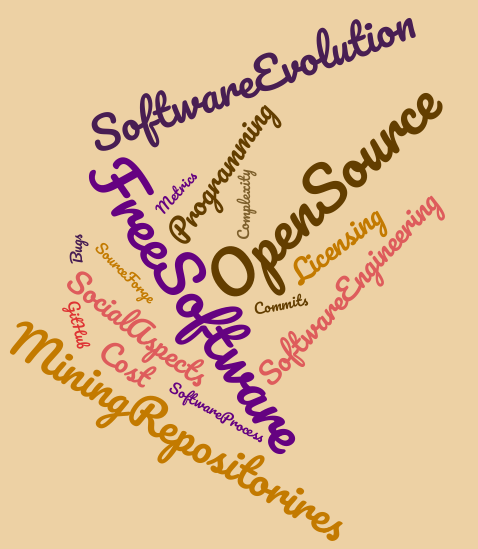
\includegraphics[width=10.4cm,height=6cm]{figs/wordcloud.png}
\end{center}
\caption{My (main) research}
\label{fig:mywordcloud}
\end{figure}

\end{frame}

\usebackgroundtemplate{}

%%--------------------------------------------------------


\begin{frame}{Overview}
\tableofcontents
\end{frame}

%%--------------------------------------------------------

\section{What is CT?}

%%--------------------------------------------------------

\usebackgroundtemplate{
\includegraphics[width=13cm]{figs/future.png}}
%background: https://www.flickr.com/photos/lendingmemo/11746994686

\begin{frame}
\frametitle{Definition of Computational Thinking}


  \begin{itemize}  
    \item Computational Thinking is the process by which a problem is formulated and a solution is expressed in such a way that a computer can carry it out effectively. (Wing, 2006)
    \item It is based on an iterative process with three stages:
    \begin{enumerate}
      \item The formulation of a problem (abstraction),
      \item the expression of a solution (implementation),
      \item and the execution and evaluation of the solution (analysis).
    \end{enumerate}
  \end{itemize}
\vspace{\baselineskip}
\vspace{\baselineskip}
\vspace{1cm}
\hfill{\Tiny Background picture: Simon Cunningham }
%
\end{frame}

\usebackgroundtemplate{}



%%--------------------------------------------------------

\begin{frame}
\frametitle{History of learning \emph{with} computers}
\begin{center}
	\begin{figure}[t!]
		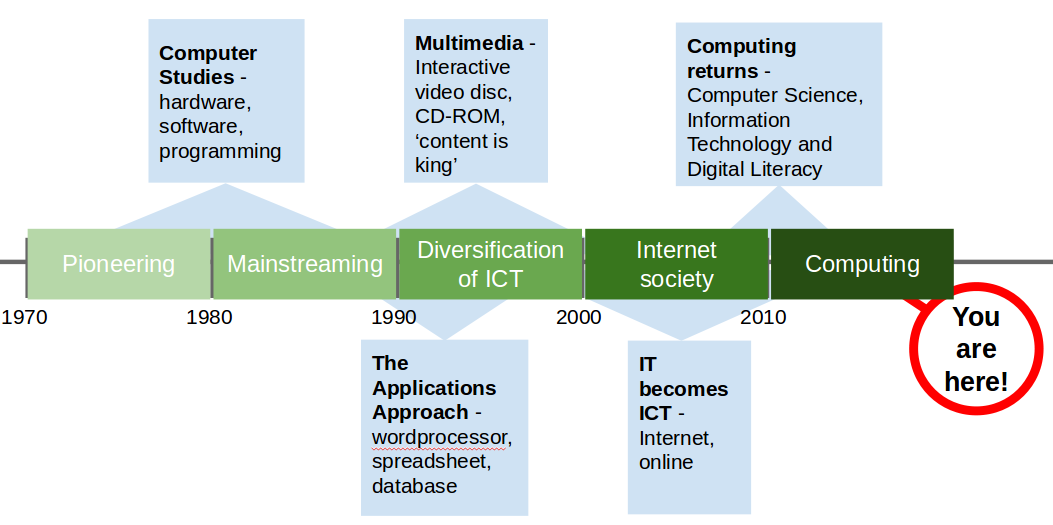
\includegraphics[width=11cm]{figs/history.png}    
    		\caption{You are here!}
	\end{figure}
	\tiny Source: \textit{REaCT EU project proposal}
\end{center}

\end{frame}

\usebackgroundtemplate{}

%--------------------------------------------------------

\begin{frame}
\frametitle{Is CT a new skill?}

\begin{figure}[htb!]
  \centering
  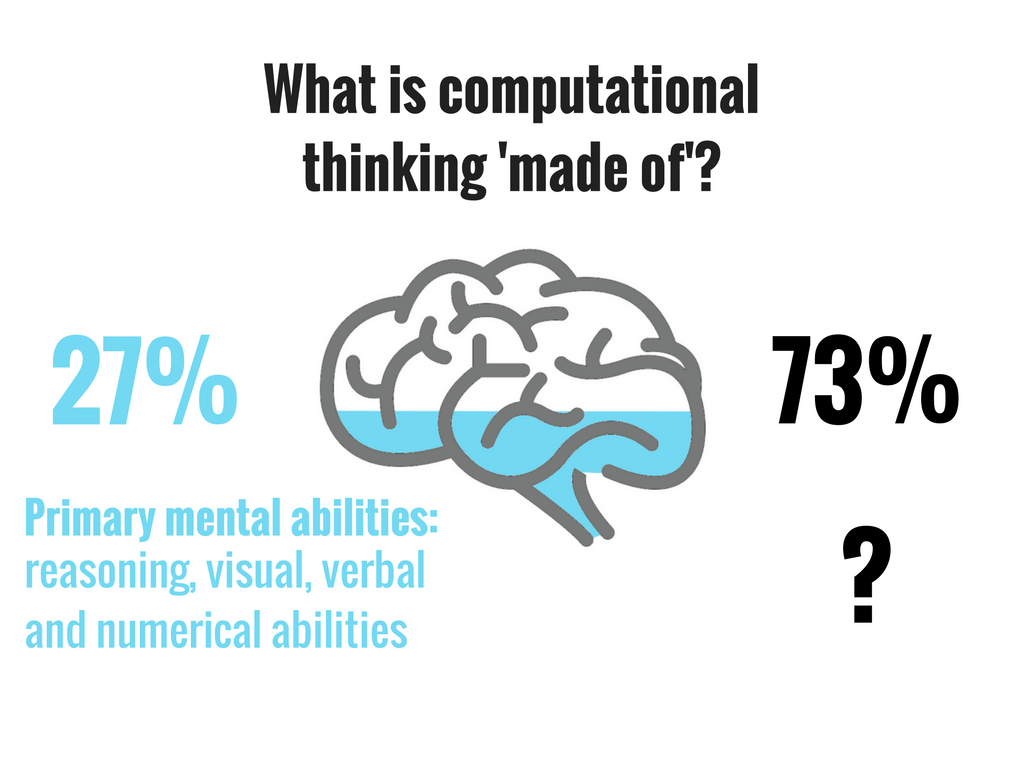
\includegraphics[width=.63\columnwidth]{figs/CT.png}
  \caption{Computational thinking is an independent skill, as only 27\% of its variance can be explained by the four primary mental abilities.}
  \label{fig:CT}
\end{figure}


\end{frame}

\usebackgroundtemplate{}


%--------------------------------------------------------

\begin{frame}
\frametitle{Impact of Research on Cognitive Effects of Programming}
\begin{center}
	\begin{figure}[t!]
		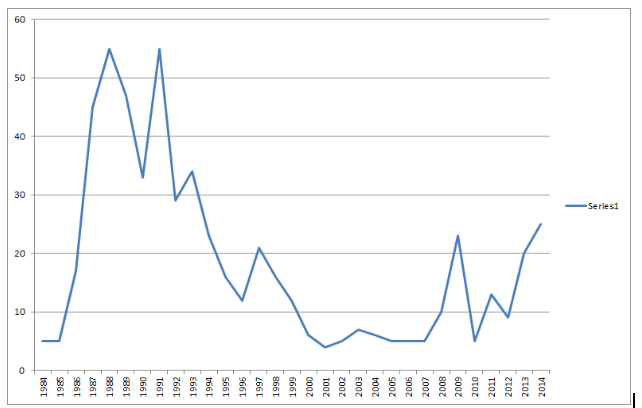
\includegraphics[width=8.8cm]{figs/citations.png}    
    		\caption{Sum of citations of 11 key papers on cognitive effects of programming 1984-2014. Calculated using Web of Science}
	\end{figure}
	\tiny Source: \textit{Nina Breshnihan, Trinity College Dublin}
\end{center}

\end{frame}

\usebackgroundtemplate{}


%--------------------------------------------------------

\begin{frame}
\frametitle{Great Principles of Computing}

  \begin{columns}[T]
    \begin{column}{0.5\textwidth}
     \begin{block}{The Book}
\begin{figure}[t!]
\begin{center}
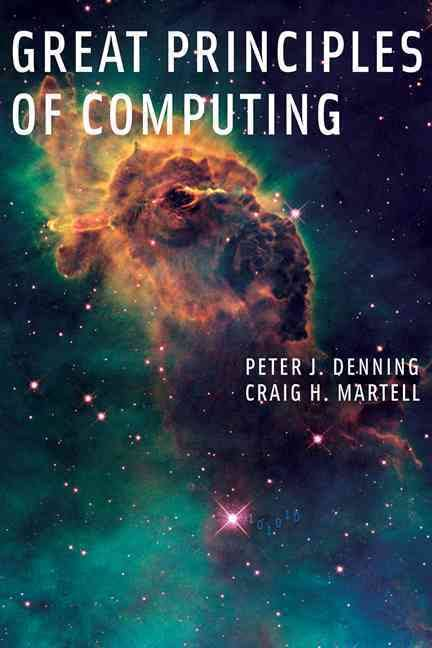
\includegraphics[width=4.4cm,height=5.6cm]{figs/gpc.jpeg}
\end{center}
\label{fig:gpc}
\end{figure}
     \end{block}
    \end{column}
    \begin{column}{0.5\textwidth}
 
     \begin{block}{Seven Principles}
\begin{enumerate}
  \item Information
  \item Machines
  \item Programming
  \item Computation
  \item Memory
  \item Parallelism
  \item Queueing
  \item and Design
\end{enumerate}
     \end{block}

    \end{column}
  \end{columns}



\end{frame}

\usebackgroundtemplate{}


%--------------------------------------------------------
%--------------------------------------------------------

\section{Learn to code}

%--------------------------------------------------------
%\usebackgroundtemplate{
\includegraphics[width=10cm]{figs/drscratch1}}

\begin{frame}
\frametitle{What is Scratch?}

An example:
\begin{center}
 {\large \url{https://scratch.mit.edu/projects/49905542/}}
\end{center}

\end{frame}

%--------------------------------------------------------
%\usebackgroundtemplate{
\includegraphics[width=10cm]{figs/drscratch1}}

\begin{frame}
\frametitle{Some fun}


\begin{center}
 {\large \url{https://scratch.mit.edu/projects/114556022/}}
\end{center}


\end{frame}


%--------------------------------------------------------
%\usebackgroundtemplate{
\includegraphics[width=10cm]{figs/drscratch1}}

\begin{frame}
\frametitle{Why automatic analysis? (Learner perspective)}

\begin{columns}[T]
    \begin{column}{1\textwidth}
     \begin{block}{Analyzing a Python program with Pylint}

\begin{figure}[t!]
\begin{center}
\begin{center}
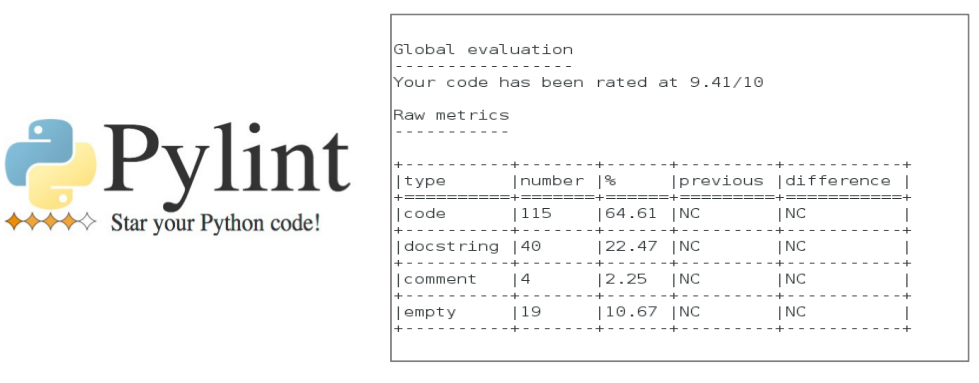
\includegraphics[width=10.5cm]{figs/pylint.png}
\end{center}
\end{center}
\end{figure}


    \end{block}
    \end{column}
  \end{columns}



\end{frame}


%--------------------------------------------------------
%\usebackgroundtemplate{
\includegraphics[width=10cm]{figs/drscratch1}}

\begin{frame}
\frametitle{Why automatic analysis? (Educator perspective)}

\begin{columns}[T]
    \begin{column}{1\textwidth}
     \begin{block}{You know what I am talking about}

\begin{figure}[t!]
\begin{center}
\begin{center}

\includegraphics[height=5.2cm]{figs/grading.jpg}
% Source: http://www.lyrics2learn.com/blog/wp-content/uploads/2014/03/Love-grading.jpg
\end{center}
\end{center}
\end{figure}


    \end{block}
    \end{column}
  \end{columns}



\end{frame}

%--------------------------------------------------------
%\usebackgroundtemplate{\includegraphics[width=13cm]{figs/iceberg.jpg}}
% background: http://www.wim-network.org/wp-content/uploads/2012/04/iceberg.jpg

\begin{frame}
\frametitle{Assessment of CT development}
\begin{table}[t]\tiny 
\centering
%\begin{tabular}{p{2.5cm}p{2.7cm}p{3cm}p{4cm}}
\begin{tabular}{|p{2cm}|p{2cm}|p{2cm}|p{2cm}|}
%\toprule
\hline
CT dimension & Basic & Developing & Proficient\\ %\midrule 
\hline
\hline  
Data representation & modifiers of sprites properties &
operations on vars & operations on lists  \\
\hline
Logical Thinking & if & if else & logic operations \\ 
\hline
User interactivity & green flag & key pressed, sprite clicked, ask and wait,
mouse blocks & when \%s is \textgreater \%s, video, audio \\ 
\hline
Algorithmic notions of flow control & sequence of blocks & repeat, forever & repeat until \\ 
\hline
Abstraction and problem decomposition & more than one script and more than one sprite & def block & clones (instances)\\
\hline
Parallelism & Two scripts on green flag & Two scripts on key pressed, two scripts on sprite clicked on the same sprite & Two scripts on when I receive message, two scripts when \%s is \textgreater \%s, two scripts on when backdrop change to \\
\hline
Synchronization & wait & Broadcast, when I receive message, stop all, stop program, stop programs sprite & wait until, when backdrop change to, broadcast and wait \\ 
\hline
\end{tabular}
\caption{Level of development for each CT dimension}
\label{table:CTscore}
\end{table}

\end{frame}


%--------------------------------------------------------
\begin{frame}
\frametitle{Assessment of CT development: Logical Thinking}

\begin{figure}[t!]
\begin{center}
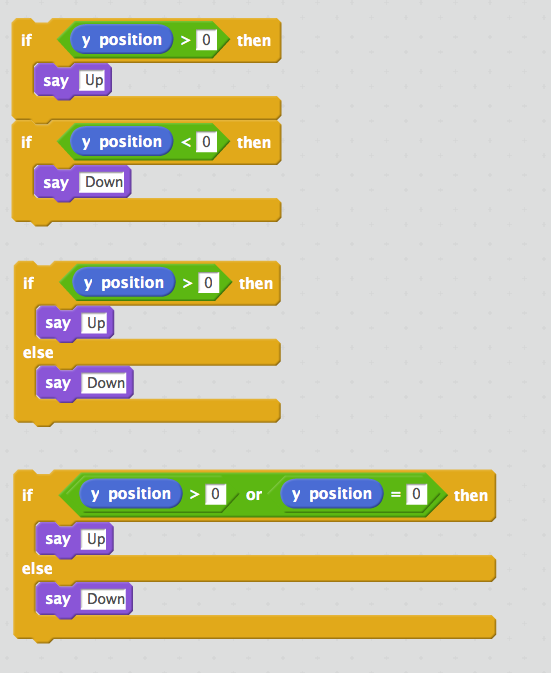
\includegraphics[height=6cm]{figs/Logic.png}
\end{center}
\label{fig:logic}
\end{figure}

\begin{center}
Different levels of development of logical thinking: basic (top), developing (center) and proficient (bottom).
\end{center}
\end{frame}

%--------------------------------------------------------
\usebackgroundtemplate{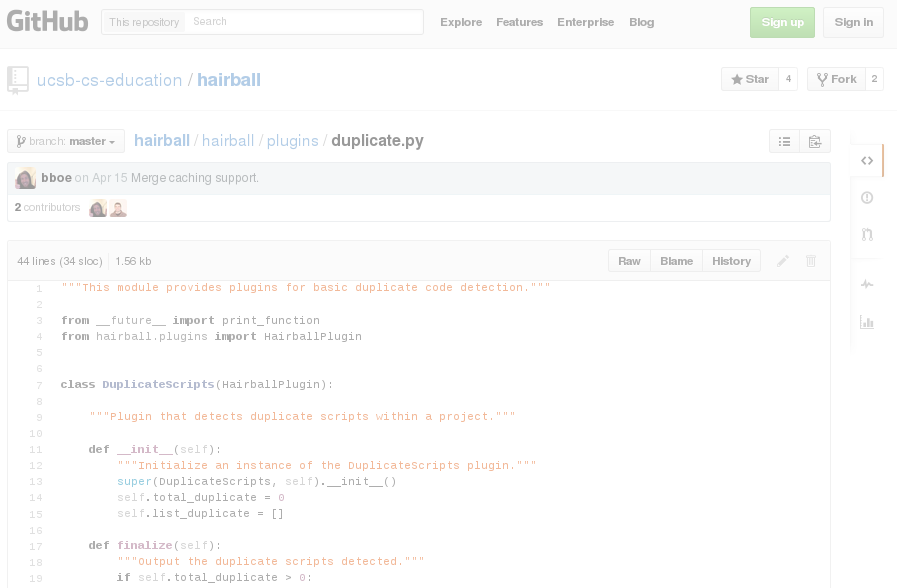
\includegraphics[width=13cm,height=9.2cm]{figs/plugins.png}}
\begin{frame}
\frametitle{Code smells (I)}
\begin{columns}[T]
    \begin{column}{0.8\textwidth}
     \begin{block}{Errors or bad programming habits}
\begin{itemize}
  \item Dead code
  \item Attribute initialization
  \item Default names
  \item Repeated scripts
\end{itemize}
    \end{block}
    \end{column}
  \end{columns}
\end{frame}

\usebackgroundtemplate{}
%--------------------------------------------------------
\begin{frame}
\frametitle{Code smells (II)}

\begin{figure}[t!]
\begin{center}
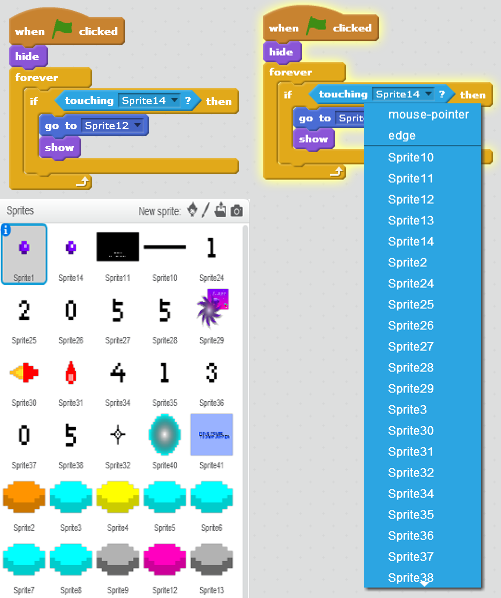
\includegraphics[width=7cm, height=6cm]{figs/SpriteNaming.png}
\end{center}
\label{fig:naming}
\end{figure}

\begin{center}
\emph{Bad}/default naming of sprites
\end{center}
\end{frame}

\usebackgroundtemplate{}
%--------------------------------------------------------

\begin{frame}
\frametitle{Code smells (and III)}

  \begin{columns}[T]
    \begin{column}{0.5\textwidth}
 
     \begin{block}{Example of repeated code}
\begin{figure}[t!]
\begin{center}
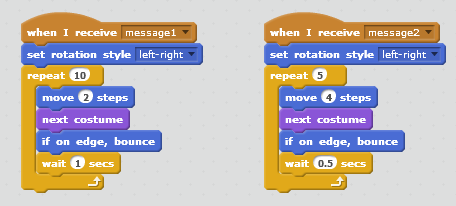
\includegraphics[width=5.4cm,height=2.5cm]{figs/CodeRepetition1.png}
\end{center}
\label{fig:repetition1}
\end{figure}
     \end{block}
    \end{column}
    \begin{column}{0.5\textwidth}
     \begin{block}{Solution to avoid repeated code}
\begin{figure}[t!]
\begin{center}
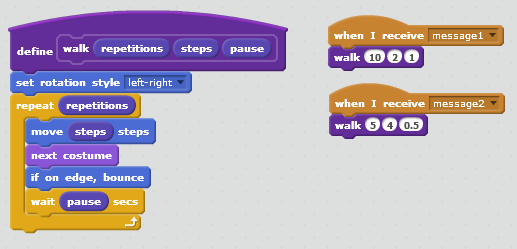
\includegraphics[width=5.4cm,height=2.5cm]{figs/CodeRepetition2.png}
\end{center}
Blocks should be created to avoid repetition of code
\label{fig:repetition2}
\end{figure}
     \end{block}

    \end{column}
  \end{columns}

\end{frame}

\usebackgroundtemplate{}


%--------------------------------------------------------
%\usebackgroundtemplate{
\includegraphics[width=10cm]{figs/drscratch1}}

\begin{frame}
\frametitle{Dr. Scratch}

\begin{figure}[t!]
\begin{center}

\includegraphics[width=9cm]{figs/drscratch1.png}
\end{center}
\label{fig:drscratch}
\end{figure}

\end{frame}


%--------------------------------------------------------
\begin{frame}
\frametitle{Feedback from/tested with learners}

\vspace{-0.55cm}

\begin{columns}[T]
    \begin{column}{1\textwidth}
     \begin{block}{Tested with learners and teachers}
\begin{center}
\begin{center}
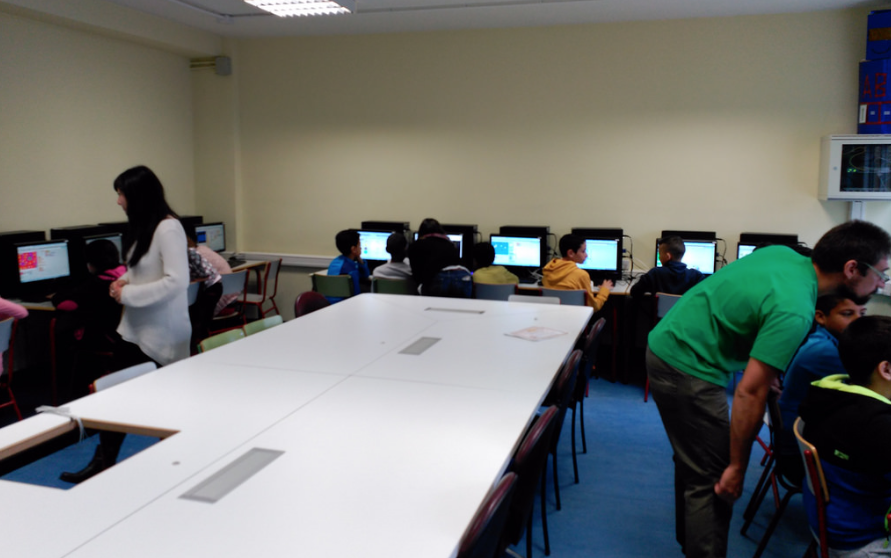
\includegraphics[height=6cm]{figs/colegio.png}
\end{center}
Workshop at CEIP Lope de Vega, Madrid (Spain)
\end{center}
    \end{block}
    \end{column}
  \end{columns}


\end{frame}

%\usebackgroundtemplate{}

%--------------------------------------------------------
\begin{frame}
\frametitle{Dr. Scratch vs classic Software Engineering Complexity (I)}
\begin{center}
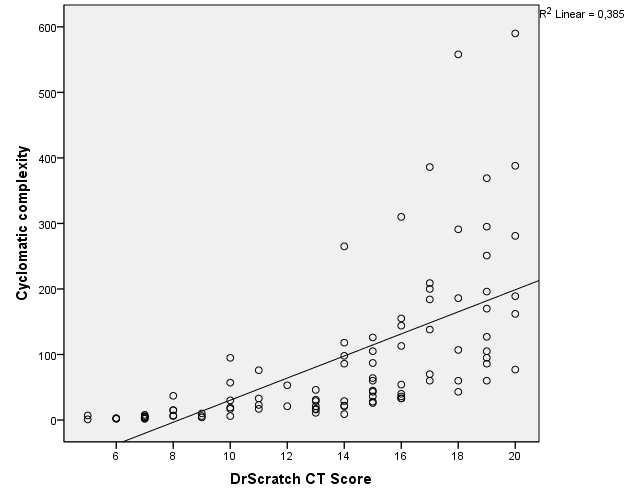
\includegraphics[height=6cm]{figs/CC.png}
\end{center}
\end{frame}

\usebackgroundtemplate{}

%--------------------------------------------------------
\begin{frame}
\frametitle{Dr. Scratch vs classic Software Engineering Complexity (II)}
\begin{center}
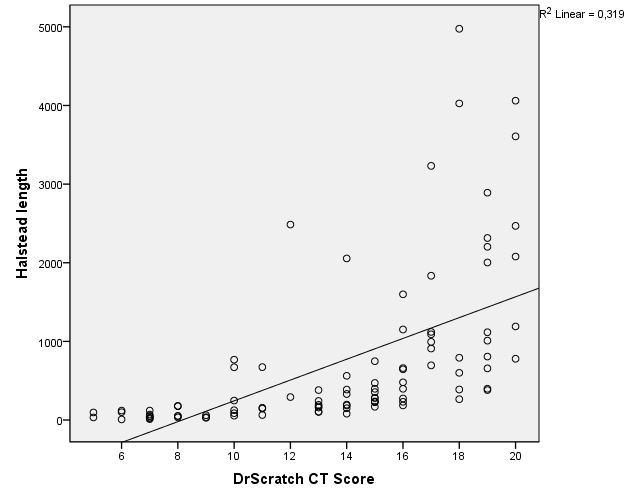
\includegraphics[height=6cm]{figs/length.png}
\end{center}
\end{frame}

\usebackgroundtemplate{}

%--------------------------------------------------------
%\begin{frame}
%\frametitle{Dr. Scratch vs Software Engineering Complexity (and III)}
%\begin{center}
%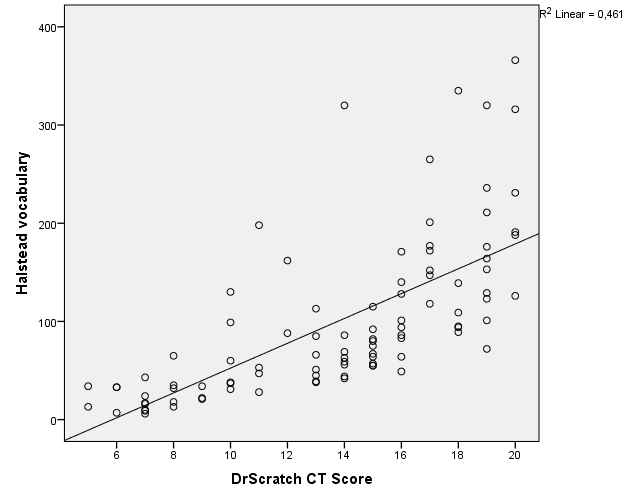
\includegraphics[height=6cm]{figs/vocabulary.png}
%\end{center}
%\end{frame}

%\usebackgroundtemplate{}

%--------------------------------------------------------
\begin{frame}
\frametitle{Dr. Scratch vs CT-test (I)}
\begin{center}
\begin{center}
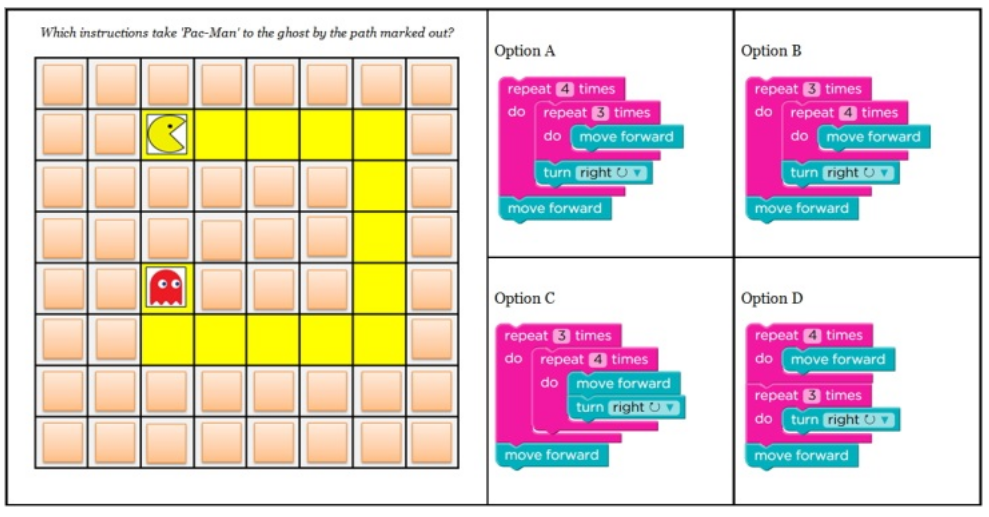
\includegraphics[height=5.9cm]{figs/comecocos.png}
\end{center}
One of the CT-test items
\end{center}
\end{frame}

\usebackgroundtemplate{}

%--------------------------------------------------------
\begin{frame}
\frametitle{Dr. Scratch vs CT-test (and II)}
\begin{center}
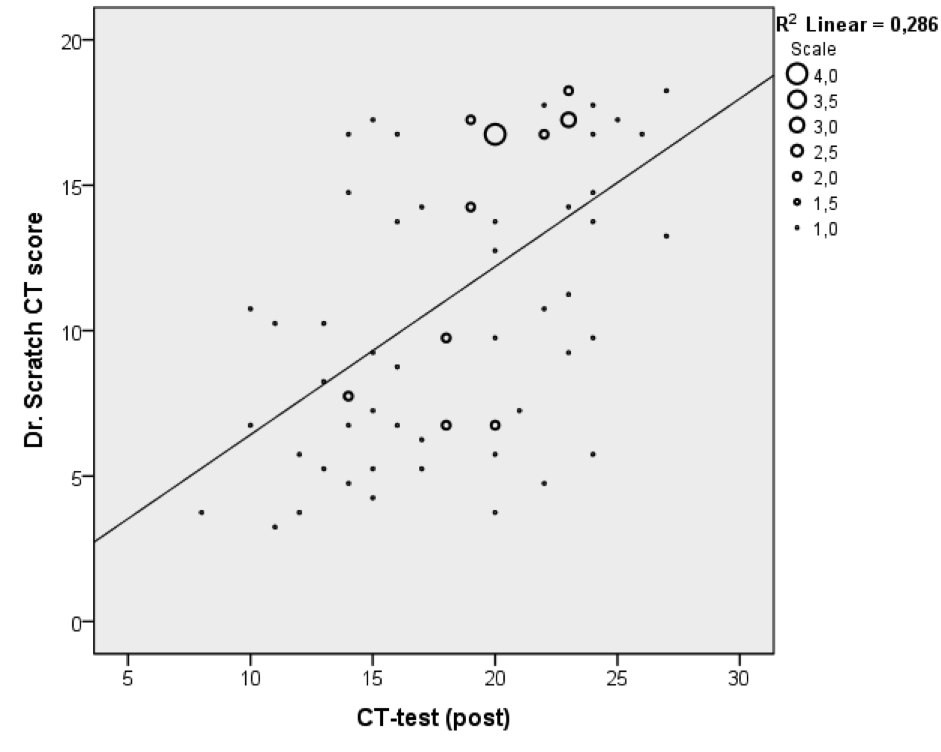
\includegraphics[height=6cm]{figs/tpc.png}
\end{center}
\end{frame}

\usebackgroundtemplate{}



%--------------------------------------------------------
\begin{frame}
\frametitle{Dr. Scratch vs Expert judgment ($r > 0.7$)}
\begin{center}
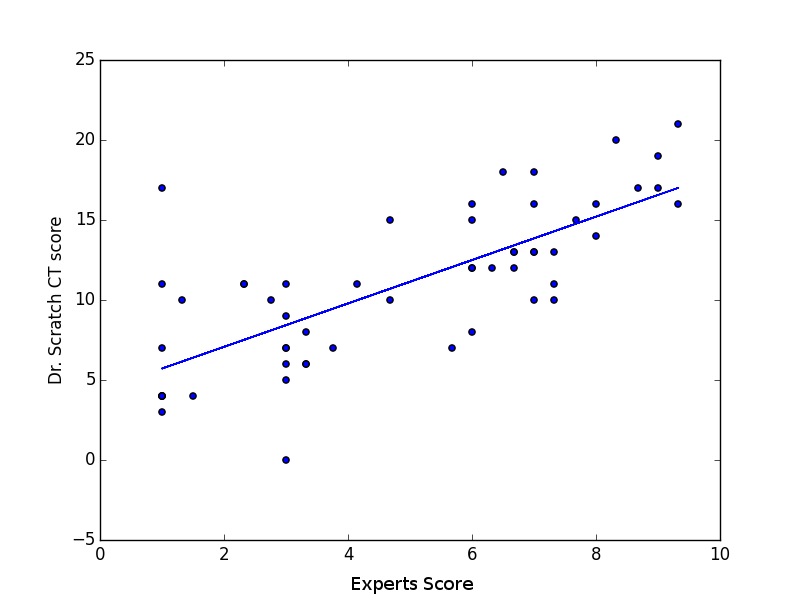
\includegraphics[height=6cm]{figs/experts.png}
\end{center}
\end{frame}

\usebackgroundtemplate{}



%--------------------------------------------------------
\begin{frame}
\frametitle{Dr. Scratch and Cheating?}

\begin{itemize} 
  \item Still work in progress
  \item Tell learners to try to obtain the highest possible score in Dr. Scratch
  \item Hypothesis: You can cheat up to your level of CT skills
\end{itemize}

\end{frame}

\usebackgroundtemplate{}


%--------------------------------------------------------
%\usebackgroundtemplate{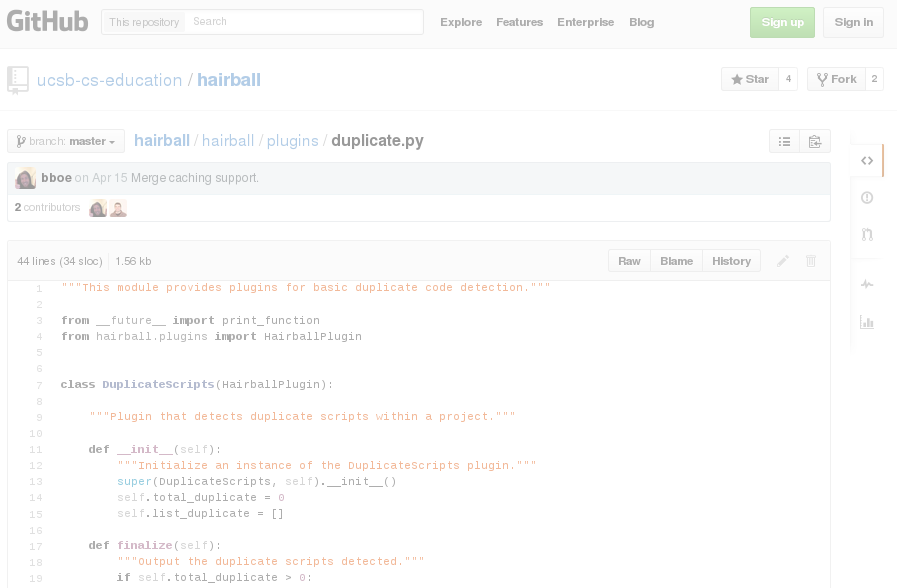
\includegraphics[width=13cm,height=9.2cm]{figs/plugins.png}}
% background: http://25.media.tumblr.com/b83aa72682992ab34b8ce7e61c0cb7f9/tumblr_menxc7qcq61ryin08o1_r1_1280.jpg
\usebackgroundtemplate{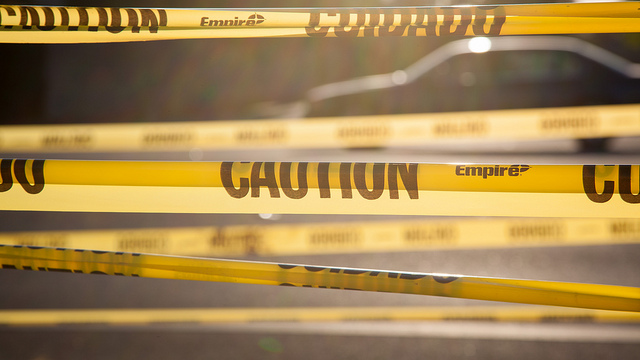
\includegraphics[width=16cm]{figs/caution.jpg}}
\begin{frame}
\frametitle{Limitations}
\begin{columns}[T]
    \begin{column}{0.8\textwidth}
     \begin{block}{Teachers should not rely exclusively on Dr. Scratch}
\begin{itemize}
  \item Fundamental CT skills are not assessed
    \begin{enumerate}
      \item Debugging
      \item Remixing (aka. Forking)
      \item Design/Modeling
    \end{enumerate}
  \item Functionality or creativity is not evaluated.
%  \item Portfolio analysis would be more accurate.
  \item Democratizing digital expression (MIT Medialab's view) may become secondary.
\end{itemize}
    \end{block}
    \end{column}
  \end{columns}
\vspace{\baselineskip}
\vspace{\baselineskip}
\hfill{\Tiny Background picture:  Robert Couse-Baker}
\end{frame}

\usebackgroundtemplate{}

    
%--------------------------------------------------------
\begin{frame}
\frametitle{Data-driven itineraries}

\begin{figure}[!t]
  \centering
    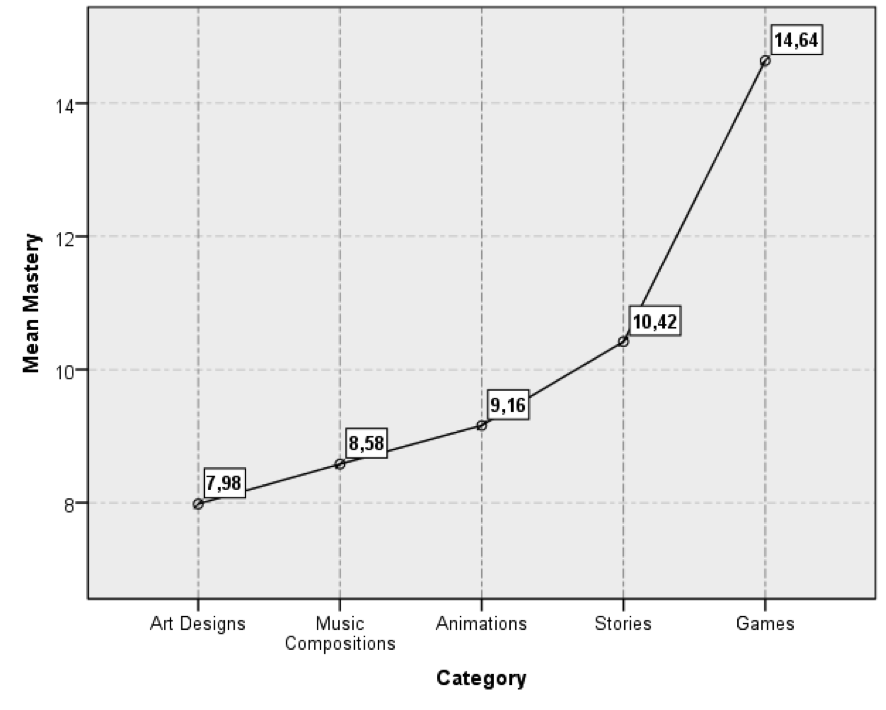
\includegraphics[width=3.5in]{figs/mastery_types.png}
  \caption{Mean of mastery score provided by \texttt{Dr. Scratch} for each category of \texttt{Scratch} projects.}
  \label{fig:mastery_types}
\end{figure} 

\end{frame}

\usebackgroundtemplate{}

%--------------------------------------------------------
\begin{frame}
\frametitle{Data-driven itineraries}

\begin{figure}[!t]
  \centering
    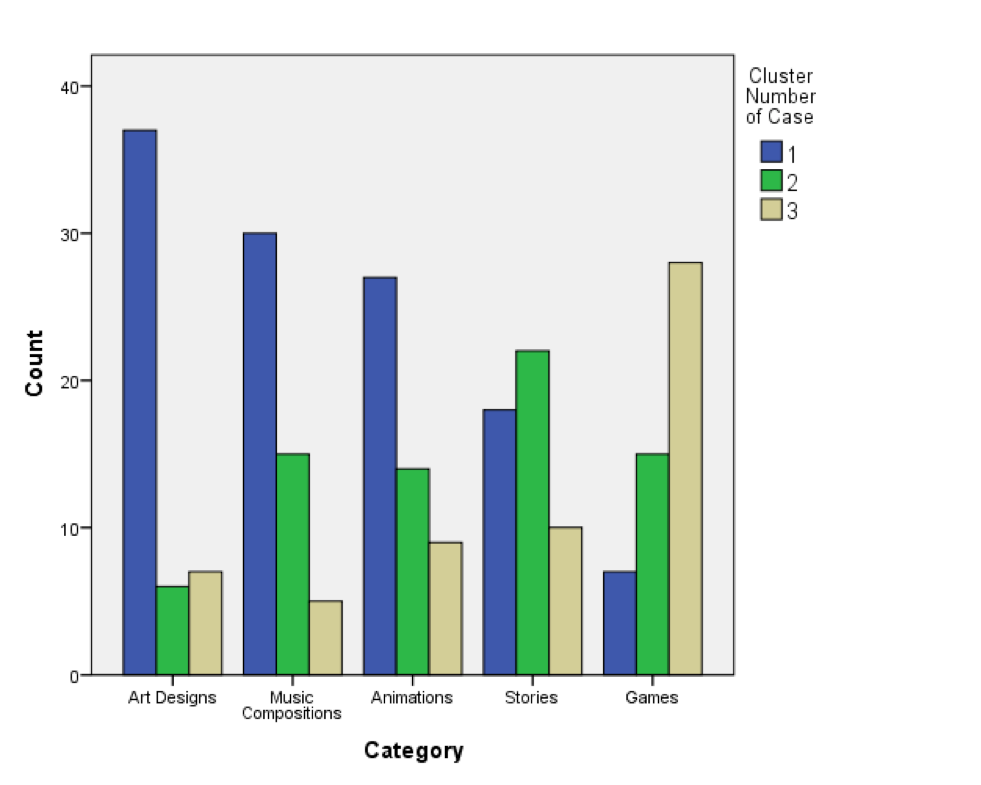
\includegraphics[width=3.5in]{figs/clusters3.png}
  \caption{Number of projects by category included in each of the three clusters of the solution.}
  \label{fig:clusters3}
\end{figure} 


\end{frame}

\usebackgroundtemplate{}


%--------------------------------------------------------
\begin{frame}
\frametitle{Does CT correlate with personality?}

\begin{itemize}
  \item Empirical evidences of the correlations between CT and the five factors of personality from the {\bf Big Five} model:
  \begin{itemize}
    \item Expected positive correlations with \emph{Openness} (r = 0.41) and \emph{Conscientiousness} (r = 0.27)
    \item Unexpected positive correlation with \emph{Extraversion} (r = 0.30)
    \item No relationship with \emph{Agreeableness} (r = 0.02) and \emph{Neuroticism} (r = 0.01)
  \end{itemize}
\end{itemize}

\end{frame}

\usebackgroundtemplate{}



%--------------------------------------------------------
\begin{frame}
\frametitle{Social learning}

\begin{figure}[h!]
\begin{subfigure}
  \centering
    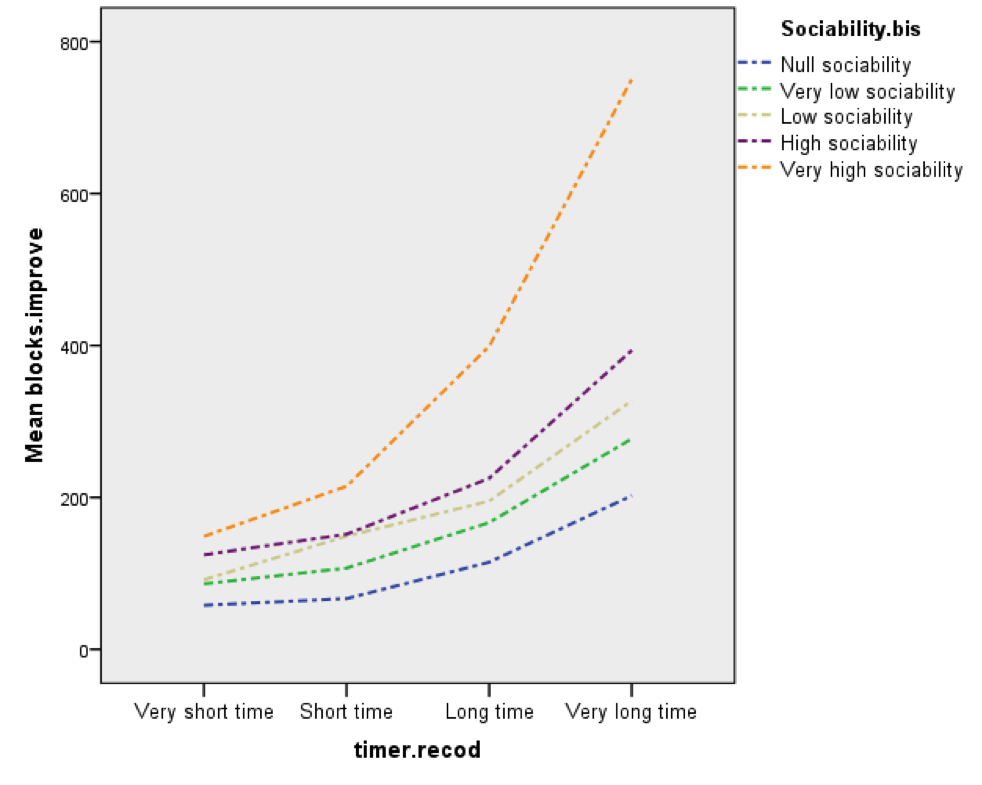
\includegraphics[width=.48\textwidth]{figs/blocks_social2.png}
\end{subfigure} 
\begin{subfigure}
  \centering
    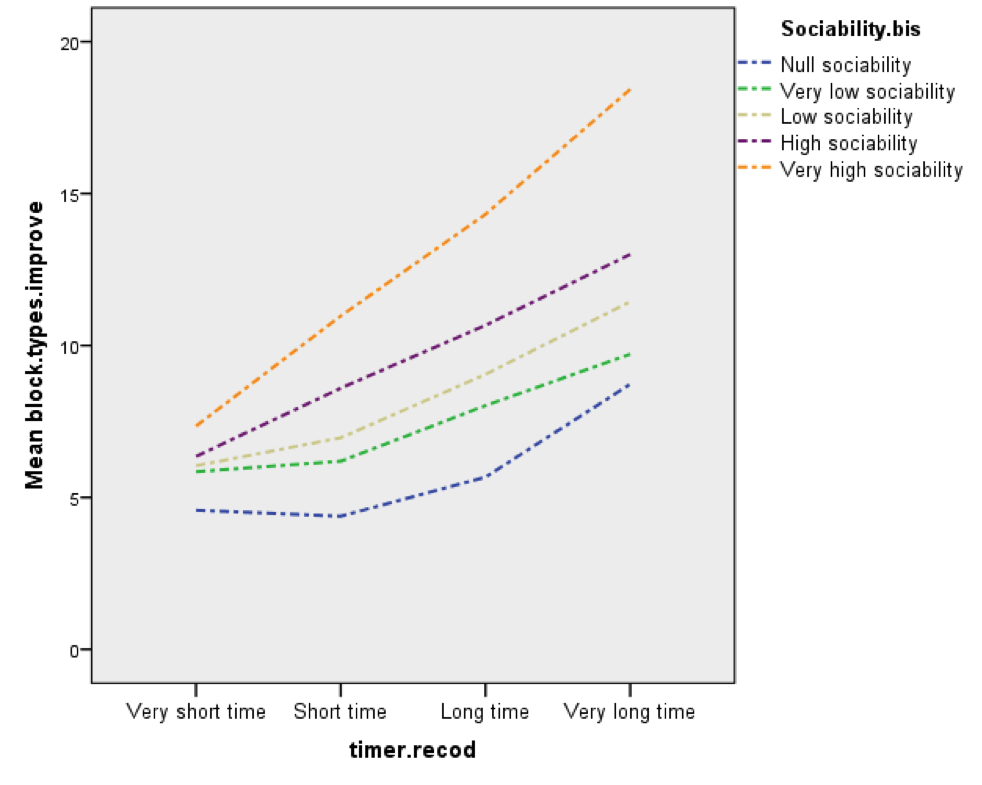
\includegraphics[width=.48\textwidth]{figs/types_social2.png}
  \caption{(l) Relationship of level of sociability with improvement in depth for each time group. (r) Relationship of level of sociability on improvement in breadth for each time group.}
  \label{fig:blocks_social2}
\end{subfigure}
\end{figure} 

\end{frame}

\usebackgroundtemplate{}

%--------------------------------------------------------
%\begin{frame}
%\frametitle{Social learning}
%
%\begin{itemize}
%  \item There is a relationship between the social conducts of
%learners in the community and the improvement in the sophistication of their
%projects
%  \item There is a relationship between the remix conducts
%of learners and the improvement in the sophistication of their projects, both in
%number of blocks, amount of types of blocks and mastery score, as very significant
%differences in the three cases in favour to the users who performed forks have been
%detected.
%\end{itemize}
%
%\end{frame}
%
%\usebackgroundtemplate{}



%%--------------------------------------------------------
\section{Code to learn}
%%--------------------------------------------------------



\usebackgroundtemplate{
\includegraphics[width=13cm]{figs/future.png}}
%background: https://www.flickr.com/photos/lendingmemo/11746994686

\begin{frame}
\frametitle{Code to learn}


  \begin{center}  
    \LARGE Computational thinking skills are not only for STEM (or for learning STEM)
  \end{center}
\vspace{\baselineskip}
\vspace{\baselineskip}

\vspace{2.5cm}
\hfill{\Tiny Background picture: Simon Cunningham }
%
\end{frame}

\usebackgroundtemplate{}

%%--------------------------------------------------------

\usebackgroundtemplate{
\includegraphics[height=8.8cm]{figs/humanities.png}}
%background: 

\begin{frame}
\frametitle{Coding beyond STEM}

\vspace{1.6cm}

  \begin{itemize}
    \item Programming is a way of expression (that is complementary to other ways of expressing yourself)
    \item Learners become \emph{prosumers}, not just consumers of technology
    \item STEM + Art = STEAM. Haven't heard about it before? 
    \item There is (preliminary) research on the (good) effects of coding in other subjects
  \end{itemize}


\vspace{1cm}
\hfill{\Tiny Background picture: ngu.edu}
%
\end{frame}

\usebackgroundtemplate{}



%%--------------------------------------------------------

\usebackgroundtemplate{}
%background: 

\begin{frame}
\frametitle{Maths}

\begin{figure}[h!]
  \centering
	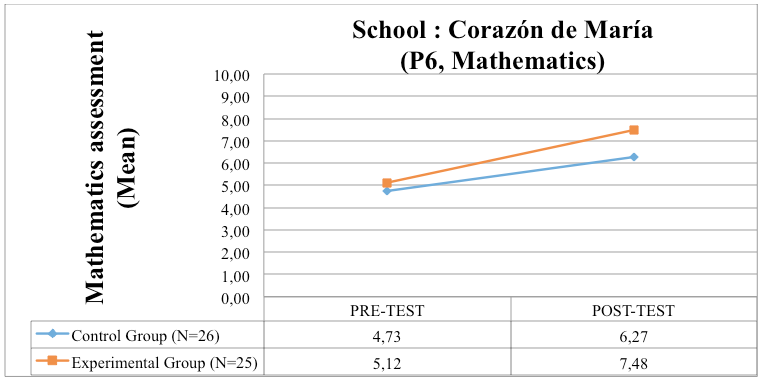
\includegraphics[width=.80\textwidth]{figs/maths.png}
  \caption{Coraz�n de Mar�a school. Comparing the improvement between pre- and post-tests of control and experimental groups.}
  \label{fig:corazon}
\end{figure}

\end{frame}

\usebackgroundtemplate{}


%%--------------------------------------------------------

\usebackgroundtemplate{}
%background: 
    
\begin{frame}
\frametitle{Social sciences}


\begin{figure}[h!]
  \centering
	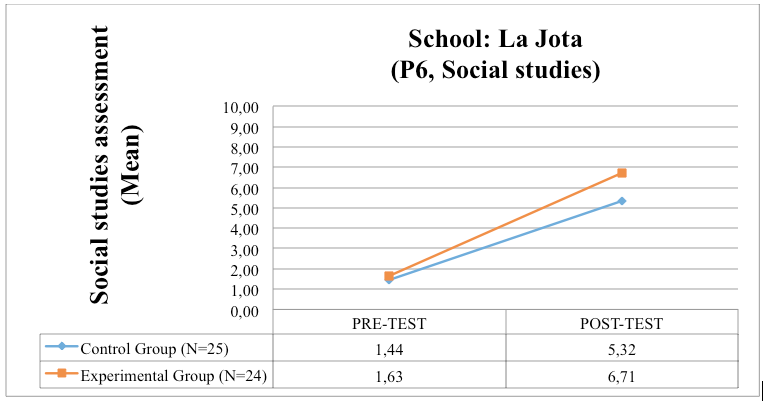
\includegraphics[width=.80\textwidth]{figs/socialstudies.png}
  \caption{La Jota school. Comparing the improvement between pre- and post-tests of control and experimental groups.}
  \label{fig:jota}
\end{figure}

\end{frame}

\usebackgroundtemplate{}

%%--------------------------------------------------------

\usebackgroundtemplate{}
%background: 

\begin{frame}
\frametitle{Arts}


\begin{figure}[h!]
  \centering
	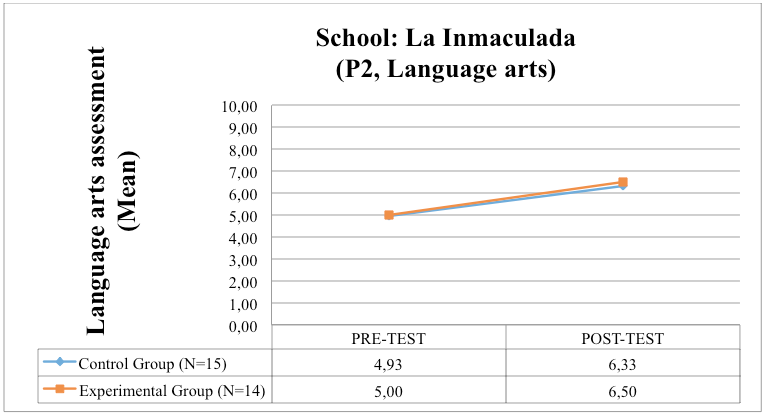
\includegraphics[width=.80\textwidth]{figs/languagearts.png}
  \caption{La Inmaculada school. Comparing the improvement between pre- and post-tests of control and experimental groups.}
  \label{fig:inma}
\end{figure}



\end{frame}

\usebackgroundtemplate{}

%%--------------------------------------------------------

\usebackgroundtemplate{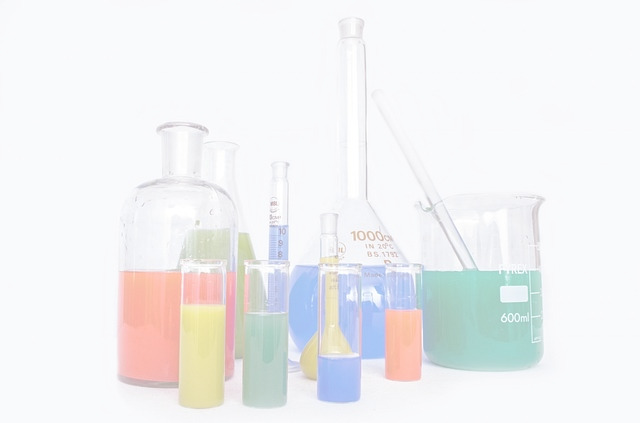
\includegraphics[height=8.8cm]{figs/research.jpg}}
%background: 

\begin{frame}
\frametitle{Research in Progress: Art with 3-year old kids}

\begin{figure}[htb!]
  \centering
  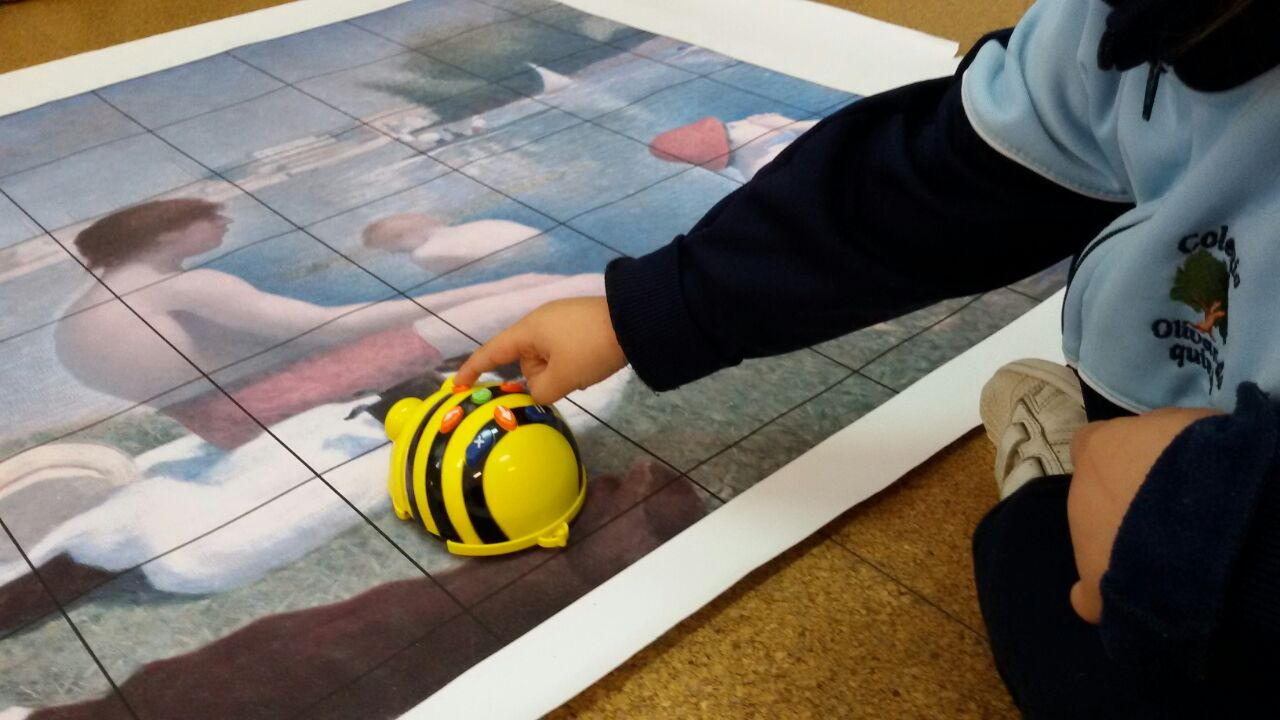
\includegraphics[width=.75\columnwidth]{figs/beebot.jpg}
  \caption{A five year old student coding a programmable robot to develop arts skills and learn about the painting \emph{Bathers at Asni�res}.}
  \label{fig:beebot}
\end{figure}



\vspace{1.5cm}
\hfill{\Tiny Background picture: Pixabay - Public domain}

\end{frame}

\usebackgroundtemplate{}



%%--------------------------------------------------------
\usebackgroundtemplate{
\includegraphics[width=13cm]{figs/take-away.jpg}}
%% background: http://flamingcow.co.uk/wp-content/uploads/2015/02/takeaway-940x283.jpg

\begin{frame}
\frametitle{Takeaways}

  \begin{enumerate}
    \item Programming in schools is back in town!
    \item But it is more than just about programming
    \item We have applied Software Engineering concepts to assess learning
    \item Based on our assessments, we have been able to look at socialization, personality and itineraries
    \item We are researching the benefits of programming in other subjects
  \end{enumerate}

\vspace{0.85cm}
\hfill{\Tiny Background picture: flamingcow.co.uk}
%
\end{frame}

\usebackgroundtemplate{}

%--------------------------------------------------------
\usebackgroundtemplate{
\includegraphics[width=13cm]{figs/books.jpg}}
% http://www.aspa-usa.org/wp-content/uploads/2015/06/books.jpg
\begin{frame}
\frametitle{Learn more}
\vspace{-0.65cm}
\begin{center}
\footnotesize
\begin{columns}[T]
    \begin{column}{1\textwidth}
     \begin{block}{Some references}
       \begin{itemize}
	 \item Moreno-Le\'on, J., Robles, G, \& Roman-Gonz\'alez, M. (2015). Dr. Scratch: Automatic Analysis of Scratch Projects to Assess and Foster Computational Thinking. \textit{RED. Revista de Educaci�n a Distancia, 15}(46).
	 \item Moreno-Le\'on, J., Robles, G, \& Roman-Gonz\'alez, M. (2016). Comparing computational thinking development assessment scores with software complexity metrics. In \textit{Global Engineering Education Conference (EDUCON), 2016 IEEE}. IEEE.
	 \item Rom�n-Gonz�lez, M., P�rez-Gonz�lez, J. C., Moreno-Le�n, J., \& Robles, G. (2016, November). Does computational thinking correlate with personality?: the non-cognitive side of computational thinking. \textit{In Proceedings of the Fourth International Conference on Technological Ecosystems for Enhancing Multiculturality} (pp. 51-58). ACM.
       \end{itemize}
    \end{block}
    \end{column}
  \end{columns}
\end{center}
\end{frame}

\usebackgroundtemplate{}



%--------------------------------------------------------
\frame{
\maketitle
\begin{center}

\includegraphics[width=2cm]{format/libresoft-logo}
\hspace{0.5cm}

\includegraphics[width=5cm]{format/gsyc-urjc}
\vspace{0.5cm}
\includegraphics[width=3cm]{format/emadrid.png}
\end{center}
}

\end{document}
